\documentclass[11pt]{sdm}
\usepackage{xcolor}
\usepackage{float}
\usepackage[utf8]{inputenc} 
\usepackage{indentfirst}
\usepackage{hyphsubst}
\usepackage[french]{babel}

%numeroter les pages
\pagestyle{plain}

\title{Software Fault Isolation using the CompCert compiler}
\author{Alexandre \textsc{DANG}}
\supervisorOne{Frédéric \textsc{Besson}}
%\supervisorTwo{No  \textsc{one}}
\team{équipe CELTIQUE}

\school{supelec}

\domain{Domaine: Cryptography and Security}

%write your abstract here
\abstract{Nous voulons durant notre stage de recherche travailler sur une problématique liée aux techniques de \textit{Software Fault Isolation}. SFI est une approche logicielle permettant d'isoler l'exécution de modules à risque et ainsi, limiter les effets de bords néfastes qu'ils pourraient introduire sur notre système. Cette bibliographie présente ainsi les différents travaux qu'on peut trouver dans l'horizon scientifique sur le domaine du SFI. Nous verrons les principes fondateurs de SFI ainsi que des adaptations de ces techniques sur différentes architectures telles que ARM ou x86. Plus particulièrement, nous nous intéresserons à une approche qui utilise le compilateur certifié CompCert qui est également l'outil que nous voulons utiliser. Nous nous inspirerons de ces travaux pour pouvoir ensuite réaliser nos objectifs durant le stage.}

\begin{document}
\maketitle

%*****************************************************************%

\section{Introduction}


Les projets informatiques sont régulièrement amenés à utiliser des modules externes dans leurs programmes. Toutefois, nous avons peu de garanties sur ces modules. En effet, rien ne nous assure qu'ils ne contiennent pas de bugs ou de code malveillant. \textit{Software Faut Isolation} est une approche qui cherche à régler cette problématique en garantissant certaines propriétés de sécurité lors de l'exécution de ces modules à risque.

Un intérêt croissant pour les techniques de \textit{Software Fault Isolation} pour les systèmes s'est fait ressentir ces dernières années dans le domaine de la sécurité. \textit{Software Fault Isolation} (SFI) est une méthode de protection de la mémoire par des moyens logiciels. L'objectif est qu'un programme protégé par SFI puisse charger dans son propre espace mémoire des modules à risque sans que ces derniers ne puissent en compromettre l'exécution. Pour cela les techniques de SFI isolent ces modules à risque dans une région de l'espace mémoire aussi appelé \textit{sandbox}. Cette opération est réalisée en réécrivant le code à risque afin qu'ils vérifient les propriétés de sécurité exigées par SFI. Ensuite ce code transformé sera analysé par un vérifieur, qui confirmera que les transformations introduites par le générateur sont bien présentes et correctement implémentées.

Les techniques de SFI sont applicables dans de nombreux domaines. Une implémentation a déjà été faite pour le navigateur web Google Chrome~\cite{Yee:2010:NCS:1629175.1629203}\cite{Sehr:2010:ASF:1929820.1929822}. En effet, des applications web s'exécutant côté client peuvent ainsi montrer des performances proches d'un code natif tout en étant isolées par des \textit{sandbox}. Les usages des techniques de SFI ne se limitent pas à ce cas, on peut également imaginer ses applications à tout système critique ayant recours à des modules externes. Par exemple des fermes de calculs qui doivent exécuter du code dont on ne connaît pas réellement l'origine ou le noyau d'un système utilisant des modules externes.

D'autres techniques de protection de la mémoire existent déjà. La plus utilisée actuellement pour isoler des modules à risque est la protection par le matériel. Les processus sont isolés dans différents espaces mémoire et ceux-ci ne peuvent interagir que par une interface d'appels systèmes bien définie. Le désavantage de cette approche est un coût relativement élevé de ces appels systèmes au niveau des performances. Ce défaut pousse certains programmes complexes à charger les modules à risque dans leur propre espace mémoire malgré les risques encourus, une problématique résolue par le SFI.

L'approche SFI comporte de nombreux avantages, ce qui explique son attrait actuel. On peut d'abord noter des performance élevées dues à l'exécution des modules à risque avec du code natif dans le même espace mémoire que le programme protégé. Un deuxième point est que, pour fonctionner, SFI nécessite une \textit{Trusted Computing Base} (TCB) relativement réduite. En effet seul le vérifieur de code qui confirme que le module à risque est bien isolé doit être impérativement de confiance (et non le générateur de code). Une TCB réduite implique que la quantité de code de confiance sur laquelle est fondée une méthode est également moindre. De ce fait, les conditions nécessaires pour que le SFI soit fonctionnel se limite uniquement au vérifieur.

Cette bibliographie va tout d'abord présenter les principes d'une approche SFI classique~\cite{Wahbe:1993:ESF:173668.168635} avec un générateur et un vérifieur comme présenté précédemment. Ensuite, nous évoquerons des travaux de recherche réalisés ultérieurement se basant sur cette approche classique, et qui adaptent les techniques de SFI pour différentes architectures dont ARM ou x86~\cite{Sehr:2010:ASF:1929820.1929822}. Finalement nous introduirons une implémentation de SFI dont l'originalité est d'utiliser le compilateur certifié CompCert~\cite{Leroy:2009:FVR:1538788.1538814}\cite{Kroll:2014:PSF:2708449.2708686}. Cette particularité nous permettra d'enlever le vérifieur des éléments du SFI et de n'utiliser qu'un générateur de code qui, couplé à CompCert garantira que le module à risque est bien \textit{sandboxé}.


\section{\textit{Software Fault Isolation} travail fondateur}



Un programme protégé par les techniques de \textit{Software Fault Isolation} aura la garantie d'être protégé des modules à risques auxquels il aura recours. Ces modules seront chargés dans son espace mémoire mais seront confinés à une zone mémoire précise aussi appelée \textit{sandbox}. Pour cela l'approche SFI est composée de deux éléments, un générateur de code et un vérifieur. Dans SFI seul le vérifieur est dans sa \textit{Trusted Computing Base}. Le générateur introduit des transformations dans le module à risque afin qu'il soit isolé dans sa \textit{sandbox}. Avant de charger le module en mémoire, le vérifieur confirmera que le \textit{sandboxing} est correctement implémenté.
Pour la suite de la bibliographie nous réserverons le terme de "programme" pour le code protégé par SFI, et "module" sera seulement utilisé pour désigner le code à risque qui sera \textit{sandboxé}.


\subsection{Principes}

Dans cette partie, nous présentons l'approche fondatrice de SFI tirée des travaux de Wahbe et al.~\cite{Wahbe:1993:ESF:173668.168635}. Les travaux ultérieurs sur SFI (cf. Section~3 et 4.2), réutilisent de nombreuses techniques que nous allons détailler dans cette partie. L'implémentation décrite ci-dessous a été réalisée dans le cas d'une architecture simple de type RISC, par exemple MIPS ou Alpha.

Pour qu'un module à risque soit correctement confiné dans sa \textit{sandbox}, le code accepté par le vérifieur SFI doit présenter les propriétés de sécurité suivantes:
\begin{itemize}
	\item \textbf{Exécution fiable}, seules les instructions qui auront été analysées par le vérifieur seront ensuite exécutées
	\item \textbf{Sûreté de la mémoire}, le module à risque ne fera ni d'écriture ni de saut hors de sa \textit{sandbox} (pour assurer la confidentialité on peut restreindre également la lecture)
	\item \textbf{Intégrité du flot de contrôle}, tous les transferts de contrôle depuis les modules à risque vers le programme protégé sont identifiés et contrôlés.
\end{itemize}

La première propriété nous garantit une protection contre du code auto-modifiant qui pourraient s'affranchir des mécanismes de protection de SFI. La propriété de \textit{Sûreté de la mémoire} protège d'une possible réécriture ou d'un accès illégal à la mémoire du programme protégé par les modules à risque. La dernière propriété permet de contrôler les interactions entre le programme et le module à risque. On empêche ainsi des appels de fonctions illégaux qui pourraient être effectués par le module à risque et qui modifieraient le flot de contrôle du programme. Une modification du flot de contrôle pourrait aboutir à une exécution non prévue par les spécifications du programme, ceci est également un comportement qu'on veut exclure avec SFI.


Le générateur modifie le code du module à risque afin que celui-ci, respecte les propriétés de sécurité citées ci-dessus. Le générateur de code est intégré dans le compilateur qui produira alors un binaire \textit{sandboxé}. Ensuite, ce binaire sera vérifié par un élément faisant partie de la TCB de l'approche SFI, le vérifieur. Son rôle est de s'assurer que les transformations de SFI sont présentes et qu'elles sont correctement implémentées au niveau des instructions dangereuses. Cette vérification se déroule juste avant que le binaire ne soit chargé en mémoire. Si la vérification n'aboutit pas, le programme sera jugé dangereux et sera rejeté par la plate-forme SFI.

\subsection{Le générateur de code}
Pour isoler le module à risque, le générateur de code va restreindre toutes ses écritures et ses sauts aux adresses de la sandbox qu'on lui a attribué.
Pour cela, le générateur de code doit faire face à trois problématiques. La première est d'installer des mécanismes de protection de ces accès, par exemple s'assurer que la destination d'un saut est une adresse autorisée. Le deuxième problème est de faire en sorte que ces mécanismes de protection ne puissent pas être contournés.
Enfin le générateur doit contrôler les interactions du module à risque vers le programme en n'autorisant que les points d'entrée spécifié par le programme protégé. Par exemple, le navigateur web Google Chrome restreint les modules qu'il utilise à une interface qu'il a défini auparavant. Le rôle des transformations SFI a pour but de restreindre les appels de fonctions, des modules vers Google Chrome, aux fonctions présentes dans l'interface.

\subsubsection{Confinement des accès mémoires}
Dans le SFI pour éviter la corruption du programme protégé par un module à risque on veut isoler le fonctionnement de ce dernier. Pour cela, on choisit de réserver une partie contiguë de la mémoire qui correspondra à la \textit{sandbox} du module à risque. La zone mémoire de la \textit{sandbox} est choisie avec une taille et une adresse de départ dont la valeur est une puissance de deux. En effet, ces particularités permettent d'utiliser des mécanismes de protection se basant sur de simples calculs au niveau des bits ce qui en accélère leur exécution. En réalité deux \textit{sandbox} sont alloués, une première pour le segment de code du module à risque et la seconde pour son segment de données.
\\
Dans ces conditions, il suffit de s'assurer que les bits de poids forts de toute adresse utilisée sont égaux aux bits de poids forts de la \textit{sandbox}. Par exemple, si on alloue à la \textit{sandbox} la zone mémoire \texttt{[0xda000000~-~0xdaffffff]}, alors toutes les adresses dont les bits de poids forts valent \texttt{0xda} appartiendront à la \textit{sandbox}. De ce fait, les transformations de SFI confineront toutes les écritures en mémoire à cette plage d'adresse. Dans notre exemple, on se limitera alors aux adresses dont les bits de poids forts sont \texttt{0xda}, cette séquence de bits est appelée \textbf{étiquette}. Cette "étiquette" permet d'identifier notre \textit{sandbox} et ce terme sera régulièrement utilisé dans le reste de la bibliographie.

Lors de la génération du code tout accès mémoire par adressage immédiat sera facilement repérable par une analyse statique. Le correctif est direct, les adresses écrites directement dans le code auront leurs bits de poids forts remplacés par l'étiquette de la \textit{sandbox}. On peut aussi décider de rejeter le programme si on estime que le code est volontairement malveillant.
Cependant le vrai problème apparaît lorsqu'une écriture ou un saut utilise un mode d'adressage indirect. En effet dans ces cas là, les adresses sont stockées sur des registres. Ainsi il est impossible de  réécrire ces adresses durant la compilation. Toutefois, pour garantir le confinement des accès mémoires dans la \textit{sandbox}, les techniques de SFI introduisent des opérations de \textit{sandboxing} dans le module à risque. 

\begin{figure}

\centering
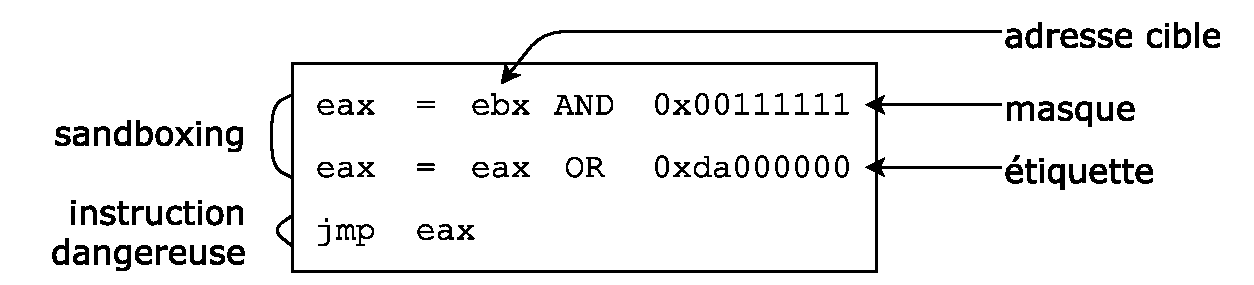
\includegraphics[scale=0.5]{images/algo_sandboxing.pdf}
\caption{Pseudo-code de l'opération de \textit{sandboxing}}
\label{fig:algo_sandbox}
\end{figure}

La Figure~\ref{fig:algo_sandbox} représente un exemple du mécanisme de \textit{sandboxing}. On peut voir que le \textit{sandboxing} est composé d'une première opération de masquage qui met à zéro les bits de poids forts de l'adresse stockée dans le registre \texttt{ebx}. Ensuite la deuxième instruction écrit l'étiquette de la sandbox sur les bits qu'on avaient réinitialisés juste avant. Ainsi l'instruction \texttt{jmp} aura une adresse de destination confinée dans la sandbox du module à risque. On peut remarquer que ce \textit{sandboxing} ne changera pas l'exécution si l'adresse ciblée était déjà dans la \textit{sandbox}. Pour l'écriture le principe est le même, on placera ces deux instructions de \textit{sandboxing} avant chaque écriture utilisant une adresse stockée sur un registre.

\subsubsection{Protection des mécanismes de \textit{sandboxing}}

On veut prévenir toute possibilité de passer outre les mesures de \textit{sandboxing} qu'on a insérées dans le code. En reprenant l'exemple de la Figure~\ref{fig:algo_sandbox} on pourrait imaginer une opération qui saute directement sur l'instruction \texttt{jmp eax}. Pour prévenir ce risque, la solution choisie est l'utilisation de registres réservés au SFI. Autrement dit, certains registres seront utilisés exclusivement pour implémenter les mécanismes de protection de \textit{sandboxing} et ne seront plus disponible pour l'exécution du code basique.
Le mécanisme de \textit{sandboxing} nécessite trois registres réservés au SFI par \textit{sandbox}. Tout d'abord nous avons besoin de conserver la valeur du masque (\texttt{0x00111111} dans la Figure~\ref{fig:algo_sandbox}). Cette valeur sera stockée sur un registre dédié au SFI qui ne pourra pas être modifié par le module à risque. De la même manière, l'étiquette identifiant la \textit{sandbox} (\texttt{0xda000000} dans la Figure~\ref{fig:algo_sandbox}) doit également être conservée dans un registre dédié pour les mêmes raisons. Le troisième registre dédié, dans notre exemple, est le registre \texttt{eax}. On force toutes les instructions de saut du module à utiliser \texttt{eax} pour référencer une adresse de destination. De ce fait, \texttt{eax} contiendra toujours des adresses de la \textit{sandbox} durant l'exécution du module.
Cette condition nous permet de confiner les sauts du module à risque dans sa \textit{sandbox}. En effet, même si les deux instructions de \textit{sandboxing} sont contournées, et qu'on exécute directement l'instruction \texttt{jmp eax}; \texttt{eax} ne contenant que des adresses de la \texttt{sandbox} on restera toujours dans celle-ci. 

On constate alors que nous avons besoin de trois registres dédiés au SFI pour le \textit{sandboxing}. Puisque nous avons une \textit{sandbox} pour le code et une seconde pour les données, une implémentation naïve nécessiterait au total six registres dédiés. Cependant, les techniques de SFI font en sorte que les deux \textit{sandbox} puissent utiliser un masque commun ce qui nous permet de réduire le nombre de registres dédiés à cinq.

Il est normal de se poser des questions quant aux performances d'une architecture à laquelle on retire cinq registres pour l'exécution du module à risque. Toutefois, dans les architecture RISC modernes incluant MIPS et Alpha on trouve en général au moins 32 registres. De plus, les différentes expériences effectuées~\cite{Wahbe:1993:ESF:173668.168635} ont montré que réduire le nombre de registres disponibles de cinq pour le compileur gcc n'impliquaient que des baisses de performances négligeables sur le temps d'exécution moyen.

\subsubsection{Contrôle des interactions avec le programme protégé}

Il est important que les techniques de SFI régulent les opérations qui permettent aux modules à risque d'interagir avec le programme principal. Sans ce contrôle, les modules à risque pourraient, par exemple, faire appel à des fonctions du programme protégé avec des paramètres erronés ce qui pourrait compromettre son état.
Pour cela, le programme protégé définit une interface qui comprend tous ses points d'entrées disponibles aux modules à risques. Cette interface indique également les paramètres autorisés pour chaque fonction de l'interface. Par exemple, comme évoqué auparavant, Google Chrome a défini une API que les modules à risque peuvent appeler pour accéder à certaines ressources du navigateur.
SFI impose alors aux modules d'accéder au programme principal par le biais de connecteurs (\textit{stubs}). Ces connecteurs sont crées par le SFI et font partie de la \textit{Trusted Computing Base} (TCB). Ceux-ci vérifient que les appels des modules à risque sont bien conformes à l'interface définie par le programme principal. Si ils le sont, le connecteur accepte la requête et la transmet au programme principal. Les appels systèmes sont également contrôlés par ces connecteurs et sont donc d'abord transférés au programme principal avant d'être transmis au noyau.
Ces connecteurs assurent aussi la sûreté des transitions entre le programme et les modules à risque. Par exemple, ils vérifient que lorsqu'on retourne dans le module, les registres dédiés ont bien les valeurs des masques, des étiquette et d'adresses appartenant à la \textit{sandbox}.

\subsection{Le vérifieur}

Le vérifieur est le dernier élément de l'approche SFI avant que le module à risque ne soit exécuté. De ce fait, il est impératif que le vérifieur fasse partie de la TCB contrairement au générateur de code. Effectivement, même si le générateur est erroné le vérifieur rejettera tout binaire qui ne sera pas conforme aux propriétés de sécurité du SFI. Cependant pour faire son analyse le vérifieur s'appuie sur le travail du générateur. L'analyse du vérifieur se contente de confirmer que les transformations du module à risque introduites par le générateur, sont présentes pour chaque instruction dangereuse et qu'elles sont correctement implémentées.
Il est possible qu'un module qui ne passe pas par le générateur ne sera pas accepté par le vérifieur, même si il respecte les propriétés de sécurité de SFI. Ce sont les transformations introduites par le générateur qui permettent au vérifieur de valider un module à risque.

Pour pouvoir analyser un binaire la première étape du vérifieur est de le désassembler. Dans l'implémentation présentée par Wahbe et al.~\cite{Wahbe:1993:ESF:173668.168635} nous nous plaçons dans une architecture MIPS ou Alpha. Dans ces architectures toutes les instructions ont une taille de 32 bits. Cette particularité nous assure que le désassemblage se fait sans encombre car il suffit de désassembler des séquences de 32 bits.
La seconde étape vérifie que le \textit{sandboxing} est correctement implémenté. Première condition, les registres dédiés au SFI contenant les masques et les étiquettes des \textit{sandbox} ne doivent jamais être modifiés. Ensuite, il reste à vérifier les registres dédiés qui contiennent les adresses de destination. Le vérifieur délimite alors dans le module à risque des régions à risque. Ces régions commencent à chaque fois qu'un registre dédié au SFI, pour les adresses de destination, est modifié. Ces régions sont fermées lorsque un saut ou une écriture avec ce registre dédié est effectué ou si il n'y a pas d'instruction après. Pour valider une région à risque le vérifieur se contente alors de confirmer qu'à la sortie de cette région le registre modifié aura une valeur valide. C'est-à-dire que le registre contiendra une adresse dont les bits de poids forts correspondent à l'étiquette de la \textit{sandbox}.

\subsection{Avantages et inconvénients}

SFI a pour but d'isoler l'exécution d'un module à risque dans l'espace mémoire virtuel d'un programme. Pour cela SFI est composé d'un générateur de code qui est chargé de produire un binaire \textit{sandboxé}. D'un vérifieur qui avant de charger le code en mémoire contrôle que celui-ci respecte bien les propriétés de sécurité de SFI. Il est primordial que le vérifieur fasse partie de la TCB pour que SFI n'accepte que du code sûr. On peut alors remarquer que pour fonctionner SFI ne nécessite pas d'avoir une grande TCB, seulement le vérifieur doit l'être ce qui est un atout. Un autre avantage est que l'approche utilisée n'est pas dépendante d'un langage. En contrepartie l'implémentation est dépendante de l'architecture dans lequel le code est exécuté, les transformations ne seront pas les mêmes sur un x86 ou sur un MIPS. Un autre désavantage de cette approche SFI est qu'en échange d'avoir un code à risque \textit{sandboxé} ses performances sont réduites et sa taille est plus conséquente. Cependant, il faut remarquer que seul les modules à risque sont modifiés et cela correspond en général à une mineure partie de l'ensemble de l'exécution. Un dernier inconvénient est que cette implémentation ne concerne que les architectures MIPS et Alpha. Cependant des travaux ultérieurs ont adapté les techniques de SFI à d'autres architectures.

  
\section{SFI pour d'autres architectures}

Dans les travaux de Wahbe et al.~\cite{Wahbe:1993:ESF:173668.168635} la méthode employée visait les architectures RISC et en particulier l'implémentation a été faite pour un processeur MIPS. Nous détaillerons maintenant les adaptations nécessaires pour les architectures x86 et ARM.

\subsection{SFI pour les architectures CISC}
	Contrairement à une architecture RISC, dans une architecture CISC les instructions peuvent être de taille variables. Cette particularité fait apparaître deux difficultés pour le SFI. Tout d'abord, il est possible pour une instruction de sauter au milieu d'une autre instruction altérant ainsi complètement le flot d'exécution. Ensuite, la phase de désassemblage du vérifieur devient beaucoup plus complexe et le code assembleur obtenu n'est pas forcément représentatif du binaire. Auparavant, avec des instructions de taille constante dans MIPS et Alpha, on avait un alignement naturel du code tous les 32 bits. Le processeur s'assurait alors que tout saut était ciblé sur une adresse respectant cet alignement de 32 bits et ainsi le programme était protégé de ce genre de fautes. Dans le cas où les instructions sont de tailles variables il est très difficile de savoir si l'adresse ciblée correspondra à l'exécution voulue et la phase de désassemblage sera aussi beaucoup moins fiable.
	
	Pour pallier ce problème, Pittsfield~\cite{Mccamant_evaluatingsfi} propose d'imposer au module à risque, un alignement artificiel en utilisant des bouts de mémoire appelées \textbf{paquets}.
Pour faire fonctionner ce modèle certaines propriétés supplémentaires doivent être respectées:
\begin{enumerate}
	\item La \textit{sandbox} est divisée en paquets dont la taille est constante et correspond à une puissance de deux
	\item Toute instruction ciblée par un saut doit se situer au début d'un paquet
	\item Tout appel de fonction doit être situé à la fin d'un paquet
	\item Il est interdit à une instruction de chevaucher deux paquets
	\item Tout paquet non rempli est complété par des instructions \texttt{no-op}
\end{enumerate}		
	
	La règle 1 nous permet de créer un alignement artificiel, ensuite la règle 2 nous permet d'avoir la propriété que toute adresse cible d'un saut respectera l'alignement. Autrement dit, en ayant des paquets de taille seize tout saut aura son adresse d'arrivée avec les quatre bits de poids faibles à zéro.
	La règle 3 assure que le retour d'un transfert de contrôle reprendra sur une instruction alignée. La règle 4 est nécessaire pour que les instructions respectent l'alignement artificiel. De ces différentes règles on peut en déduire une propriété d'atomicité d'un paquet. Plus précisément, sachant qu'il est impossible de sauter au milieu d'un paquet nous pouvons alors en déduire que les instructions d'un même paquet s'exécuteront toujours de manière atomique.
	Cette propriété d'atomicité des paquets nous apporte un grand gain, celle-ci nous permet de nous affranchir des registres réservés au SFI. Effectivement, ces derniers étaient utilisés pour empêcher de contourner les opérations de \textit{sandboxing}. En profitant de l'atomicité des paquets on peut alors s'assurer que le \textit{sandboxing} d'un saut ou d'une écriture ne peut pas être évité par un saut directement sur l'instruction dangereuse. Pour cela, il suffit que le générateur de code place les instructions de \textit{sandboxing} dans le même paquet que l'instruction qu'il confine. Les mécanismes de protection de \textit{sandboxing} ne pouvant plus être contournés, nous ne sommes plus obligés d'utiliser des registres dédiés. 
	Le point faible de cette approche est une diminution des performances du module à risque due à l'alignement artificiel imposé. Les bancs de test réalisés nous indiquent une baisse des performances moyennes de 21\% par rapport à une exécution non-modifié du module à risque.


\subsection{NativeClient l'implémentation de SFI par Google}

Google a développé Native Client~\cite{Yee:2010:NCS:1629175.1629203} qui est aujourd'hui inclut par défaut dans son navigateur Google Chrome. Celui-ci utilise du SFI pour pouvoir exécuter des modules à risque dans Google Chrome, ces modules qui sont exécutés nativement montrent des performances plus élevés qu'avec le JavaScript.
NativeClient est certainement la mise en œuvre la plus aboutie de SFI. 

\subsubsection{NativeClient pour x86-32}

La première version de NaCl (Native Client) a été développée pour une architecture x86-32~\cite{Yee:2010:NCS:1629175.1629203}. Cette implémentation combine l'utilisation des segments mémoires x86 avec des idées de l'approche précédente sur les architectures CISC. Pour que NaCl respecte les exigences de sécurité imposée par SFI, l'équipe de Google a mis en place plusieurs règles de construction présentées dans la Figure~\ref{nacl_constraints}.

\begin{figure}
\centering
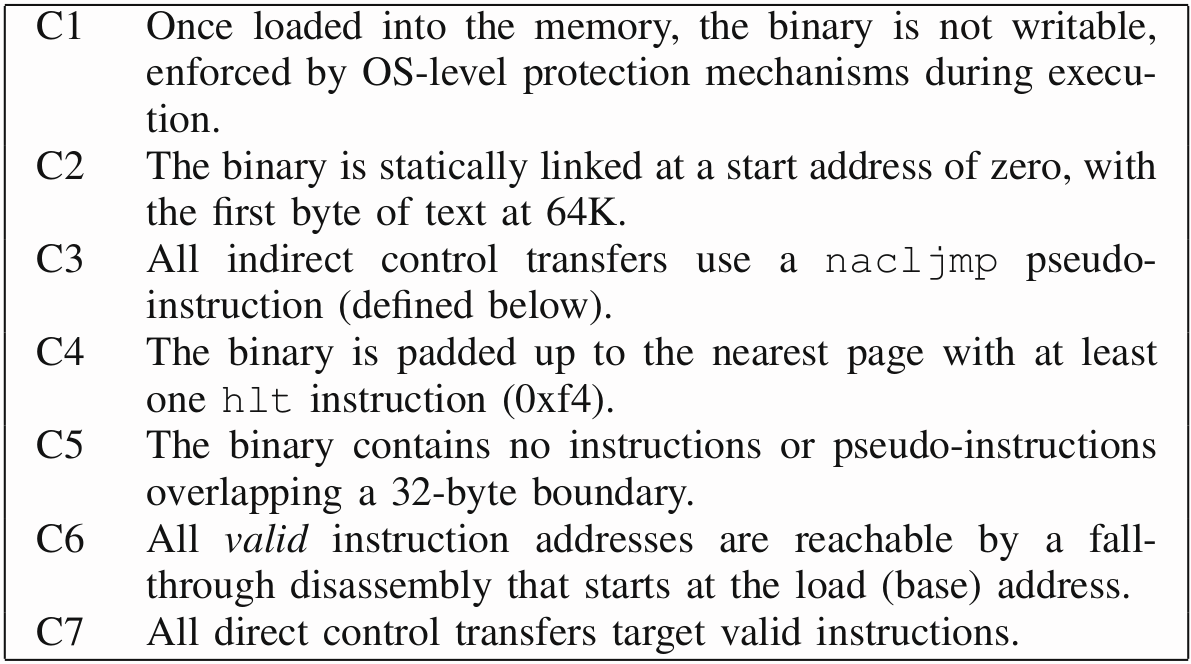
\includegraphics[scale=0.25]{images/nacl_constraints.png}
\caption{Règles de construction d'un module NaCl (Bennet Yee et al.~\cite{Yee:2010:NCS:1629175.1629203}, Table~1)}
\label{nacl_constraints}
\end{figure}

NaCl se sert des segments mémoires x86 pour restreindre les références sur les données dans un espace mémoire contig\"ue. Cela signifie que ces segments mémoires x86 nous permettent de confiner les écritures et les lectures dans la \textit{sandbox} sans avoir à implémenter les opérations de \textit{sandboxing}. Cette méthode nous permet de gagner beaucoup en temps d'exécution et en taille de code.

Ensuite il faut confiner les autres instructions dangereuses dans la \textit{sandbox}. Pour restreindre les adresses de destination des sauts, NaCl utilise le segment \texttt{CS} qui est un segment de code. On impose à celui-ci de commencer son adressage à partir de l'adresse 0 comme l'indique la règle C2 de la Figure~\ref{nacl_constraints}. Ainsi n'ayant qu'à mettre les bits de poids forts à zéro on peut réduire l'opération de \textit{sandboxing} à deux instructions au lieu de trois comme on peut le voir dans la Figure~\ref{nacl_jump}. De plus l'opération assure que l'adresse ciblée est alignée sur un multiple de 32, cette technique étant inspirée de l'approche par paquet d'instructions vue auparavant (règle C5 de la Figure~\ref{nacl_constraints}). Cette opération est nommée \texttt{nacljmp} par NaCl (règle C3 de la Figure~\ref{nacl_constraints}).

\begin{figure}[b]
\centering
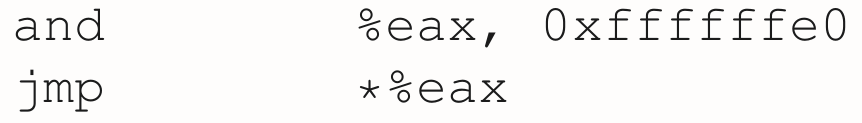
\includegraphics[scale=0.22]{images/nacl_jump.png}
\caption{\textit{Sandboxing} réduit en \texttt{nacljmp}(Bennet Yee et al.~\cite{Yee:2010:NCS:1629175.1629203})}
\label{nacl_jump}
\end{figure}

%La règle C4 permet d'implémenter la technique d'optimisation qui consiste à placer des zones de gardes aux frontières des segments afin de se protéger des accès mémoires avec biais. 

On peut remarquer que les règles C1 et C6 de la Figure\ref{nacl_constraints} assurent que la phase de désassemblage du binaire est fiable. C1 en particulier permet à NaCl de se prémunir des programmes auto-modifiants. Si ceux-ci étaient acceptés ils rendraient les méthodes de SFI obsolètes.
De ce fait par un désassemblage fiable NaCl respecte la propriété énoncé au début, que seules les instructions qui auront été analysées seront ensuite exécutées. Cette propriété essentielle au fonctionnement de SFI est très rarement évoqué dans les autres travaux et NaCl est la seule qui l'implémente explicitement.

NaCl fait également le choix d'interdire les appels systèmes, les instructions qui peuvent modifier l'état des segments et remplace l'instruction de retour \texttt{ret} par un \texttt{pop} de la pile suivi d'un \texttt{nacljmp} sur l'adresse de retour qui sera préalablement stockée dans un registre. Cette dernière manipulation nous permet de nous protéger d'une faille de l'instruction \texttt{ret}. Celle-ci utilise pour son transfert de contrôle l'adresse sauvegardée dans la pile (plutôt qu'une valeur dans un registre), de ce fait elle est vulnérable à la concurrence des \textit{threads}. En effet rien ne nous garantit que la valeur utilisée sera toujours la même que celle qui a passé les vérifications (\textit{Time Of Check Time Of Use}).


\subsubsection{NativeClient pour x86-64 et ARM}
NaCl voulant être utilisé avec le navigateur Google Chrome, Google a fait évoluer son produit vers les architectures les plus courantes actuelles qui sont x86-64 et ARM (smartphones). Ces deux versions de NaCl sont des versions de NaCl-x86-32 adaptées aux spécificités de ARM et x86-64. Par exemple, ces deux architectures ne contiennent pas de segments mémoires et de ce fait, NaCl est forcé de revenir sur un \textit{sandboxing} plus classique pour les écritures.
Ces deux implémentations n'apportant pas d'idées nouvelles au SFI nous ne détaillerons pas leur implémentation ici mais plus d'informations peuvent être trouvés dans leurs travaux~\cite{Sehr:2010:ASF:1929820.1929822}.

Pour conclure sur NaCl, les deux implémentations ont montré durant les tests des baisses de performance moyennes de 5\% pour ARM et 7\% pour x86-64. Ces résultats très satisfaisants prouvent qu'une implémentation de SFI sur les architectures modernes est viable pour exécuter du code à risque de manière native dans un navigateur. Comme cité auparavant, NativeClient est déjà inclut dans Google Chrome et il est possible de tester NaCl en téléchargeant dans le web store de Google des applications compatibles telles que Quake qui est un classique des jeux vidéos.

\section{SFI avec un compilateur certifié}


Jusqu'à présent nous n'avons vu que des implémentations de SFI basées sur le modèle traditionnel: un générateur de code puis un vérifieur de code faisant partie de la TCB. Une approche possible que nous allons présenter est celle du compilateur certifié. En effet, celui-ci a la particularité que le code qu'il produit gardera la sémantique du code source. De ce fait il est possible de faire les transformations SFI sur un code de plus haut niveau et avoir la garantie que le code assembleur produit en sortie conservera les propriétés de sécurité introduites dans le code de haut niveau.
Nous nous intéresserons plus particulièrement au compilateur certifié CompCert~\cite{Leroy:2009:FVR:1538788.1538814} et de son utilisation pour implémenter le SFI.
Cette partie est particulièrement intéressante dans le cadre de notre bibliographie sachant que CompCert est l'outil que nous voulons utiliser pour faire du SFI. Nous nous inspirerons certainement de certains éléments de ce travail pour implémenter nos solutions et notamment les techniques de transformation SFI sur le modèle de mémoire de CompCert.

\subsection{CompCert compilateur certifié pour le langage C}

\subsubsection{CompCert}

CompCert est un compilateur certifié qui supporte presque tout le C défini par ISO C 99. Ce compilateur peut produire du code pour les différentes architectures PowerPC, ARM et x86-32. Sa particularité est d'avoir été formellement prouvé et écrit avec l'assistant à la preuve Coq. Ce sont ces preuves qui nous permettent d'avoir confiance en la conservation de la sémantique au fil des passes de compilation de CompCert.

\begin{figure}
\centering
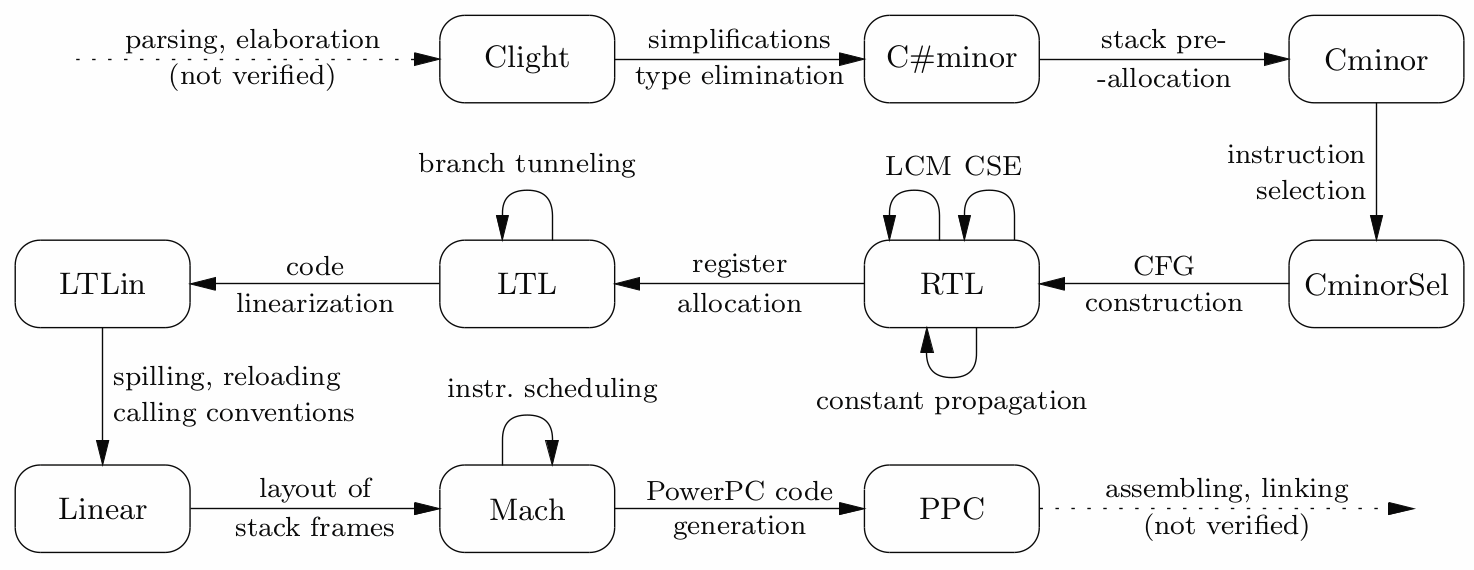
\includegraphics[scale=0.32]{images/compcert_pass.png}
\caption{Passes de compilation et langages intermédiaire de CompCert (Xavier Leroy~\cite{Leroy:2009:FVR:1538788.1538814}, Figure~1)}
\label{compcert_passes}
\end{figure}

CompCert a un schéma de compilation standard pour un compilateur comme on peut le voir sur la Figure~\ref{compcert_passes}. Il présente quelques optimisations classiques telles que la propagation de constantes ou l'élimination des sous-expressions communes. Les performances du code produit par CompCert sont correctes, sur PowerPC on atteint 90\% des résultats de gcc avec une optimisation de niveau 1.

CompCert respecte un théorème de correction qui garantit que tout programme compilable par CompCert conservera sa sémantique. Plus précisément, tout programme source $S$ sémantiquement bien défini dans CompCert sera compilé en un code assembleur $C$ qui vérifie les mêmes propriétés que $S$. Un programme qui n'est pas sémantiquement bien défini signifie qu'il ne respecte pas la sémantique opérationnelle établie par CompCert. Dans ce cas là, CompCert ne donne aucune garantie sur la sémantique du programme qui sera produit. Une opération n'ayant pas de sémantique dans CompCert est par exemple, un accès hors des bornes d'un tableau.

\subsubsection{Modèle mémoire de CompCert}

Dans CompCert une représentation abstraite de la mémoire est utilisé~\cite{compCert_memory_model}. Celle-ci est utilisée pour prouver la conservation de la sémantique dans les différentes passes de compilation. De ce fait, tous les langages intermédiaires de CompCert partagent ce modèle commun de la mémoire. La mémoire est représentée par des blocs de taille finie et ces blocs sont attribués un numéro $b$. Ces blocs sont disjoints et pour accéder aux adresses contenues dans ces blocs on utilise un offset $\delta$. Les pointeurs sont donc représentés par le couple $(b,~\delta)$. Il est également possible d'avoir des pointeurs de fonctions, ceux-ci sont représentés par des blocs de code ayant des adresses de bloc $b$ négatives.
Il peut-être surprenant qu'une représentation si abstraite de la mémoire donne un contrôle assez fin pour pouvoir utiliser les techniques de SFI. Cependant, le fait que les blocs de mémoires soient disjoints est suffisant pour isoler une région de la mémoire. Ainsi, pour confiner le module à risque dans une \textit{sandbox} nous confinerons ses accès mémoires à un des blocs mémoire de CompCert qui sera notre \textit{sandbox}.


\subsection{SFI avec CompCert}

Nous allons présenter une implémentation de SFI avec CompCert qui a été faite par Joshua A. Kroll, Gordon Stewart et Andrew W. Appel~\cite{Kroll:2014:PSF:2708449.2708686}.
 L'approche est divisée en deux parties, tout d'abord les transformations SFI s'effectuent sur un langage intermédiaire de CompCert qui est Cminor. On obtient alors un code Cminor \textit{sandboxé} qui vérifie les propriétés de sécurité de SFI. Le théorème de correction de CompCert implique alors, que si ce Cminor \textit{sandboxé} est sémantiquement bien défini, alors le code assembleur produit respectera également les propriétés de sécurité de SFI.
 De ce fait, le vérifieur, usuellement présent dans SFI, n'a plus lieu d'être puisque CompCert apporte les mêmes garanties que ce dernier. On en déduit alors, que cette approche de SFI aura une TCB allégée du vérifieur, ce qui est un avantage.

\subsubsection{Cminor}
Cminor est un langage intermédiaire crée pour CompCert, il est semblable à du C simplifié auquel on enlève le typage des variables.
Le choix de Cminor pour SFI n'est pas anodin, en effet c'est le langage de plus bas niveau dans la chaîne de compilation de CompCert qui est indépendant de l'architecture ciblée. Ainsi, les transformations SFI effectuées sur Cminor seront portables sur toutes les architectures que CompCert peut servir.
De plus Cminor est assez bas niveau pour être la cible de nombreux langages de programmation qui veulent entrer dans la chaîne de compilation de CompCert.
%Cminor possède une sémantique opérationnelle petit pas qui est utilisé pour estimer la cohérence du programme  
Pour ces différentes raisons Cminor est le candidat idéal pour les opérations de \textit{sandboxing} de SFI.

\subsubsection{Spécifications de la transformation SFI}

Les techniques de SFI doivent généralement garantir la condition suivante. Une implémentation de SFI doit être capable de transformer n'importe quel module à risque en un module qui respecte les propriétés de sécurité exigées par l'approche SFI. De ce fait, même pour un module à risque qui n'est pas sémantiquement bien défini, l'approche CompCert-SFI doit quand même produire un code vérifiant les propriétés de sécurité de SFI.
 De ce fait il faut que le Cminor \textit{sandboxé} respecte les deux propriétés suivantes:
\begin{itemize}
	\item le Cminor \textit{sandboxé} confine tous les accès en mémoire à la \textit{sandbox} qui lui est dédié
	\item le Cminor \textit{sandboxé} doit être sémantiquement bien défini pour que le théorème de correction puisse être appliqué
\end{itemize}

De ce fait, si le code source n'est pas sémantiquement bien défini les transformations SFI doivent lui donner une sémantique dans CompCert, même si son comportement s'en retrouve modifié. Toutefois SFI doit également respecter que si un module à risque respecte déjà les propriétés de sécurité de SFI, les transformations appliquées ne changeront pas son comportement.


\subsubsection{Masquage dans CompCert}

L'approche SFI-CompCert se sert du modèle mémoire par bloc de CompCert pour isoler le module à risque dans un unique bloc. Pour cela, SFI utilise habituellement un procédé de masquage des bits de poids forts pour confiner les adresses utilisées dans la \textit{sandbox}. Cependant, lors de la publication de cet article, Cminor n'avait pas de sémantique pour l'arithmétique de pointeurs et il était alors impossible de faire le \textit{sandboxing} traditionnel dans ce langage. Pour pallier ce problème, la solution trouvée a été de créer une fonction \textit{mask} qui a été intégrée dans CompCert. Cette fonction \textit{mask} a été axiomatisée pour pouvoir prouver qu'elle ne changeait pas la sémantique du programme dans le cas où les accès mémoire restaient bien dans la \textit{sandbox}. Par exemple, \og si la variable d'entrée contient un pointeur pointant sur le bloc SFI alors sa valeur est inchangée au retour de la fonction\fg{} est un des axiomes de \textit{mask}.

\begin{figure}
\centering
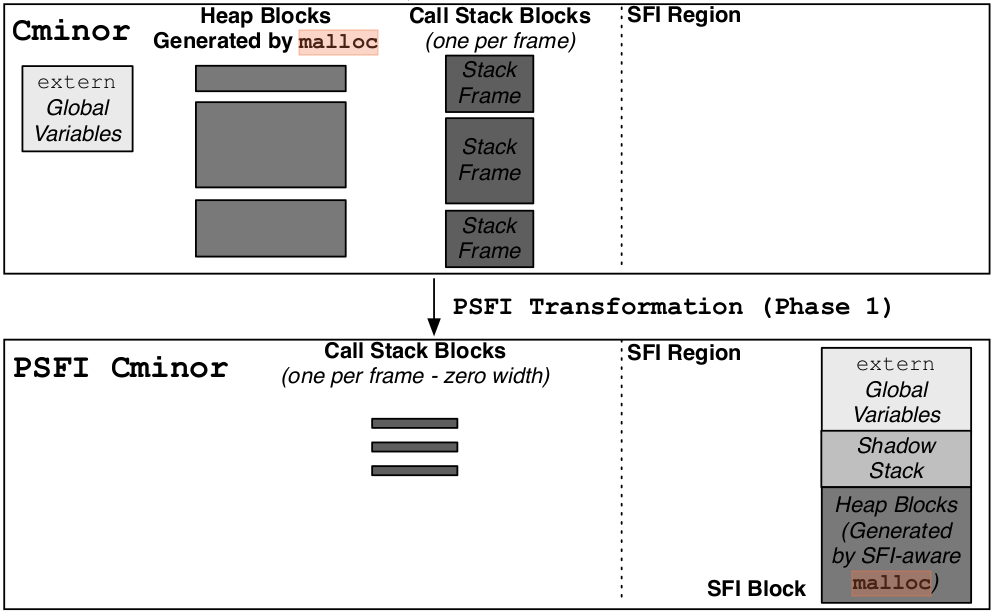
\includegraphics[scale=0.36]{images/psfi.png}
\caption{\textit{Sandboxing} du module à risque dans un bloc mémoire de CompCert (Joshua A. Kroll et al., Figure~1)}
\label{psfi}
\end{figure}

\subsubsection{Transformations SFI}

Il existe deux manières dans CompCert d'allouer de la mémoire, la première est d'appeler une fonction observable externe telle que \texttt{malloc} sinon il faut empiler de nouvelles trames sur la pile.
La transformation SFI se base sur ces données et effectue plusieurs passes de transformations qui sont présentées ci-dessous.

\begin{itemize}
	\item \textit{Construction d'une pile secondaire}, permet de s'assurer que les variables locales de la pile ne soient accédées que dans la région de mémoire SFI. On crée une pile secondaire dans la région SFI qui sera construite par des \texttt{malloc}s. Un exemple est illustré dans la Figure~\ref{shadow_stack}.
	
	
\begin{figure}[b]
\centering
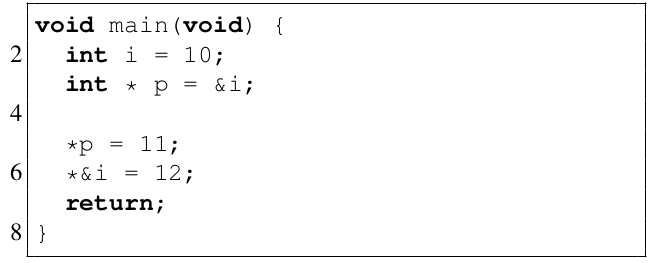
\includegraphics[scale=0.33]{images/before_shadow.png}
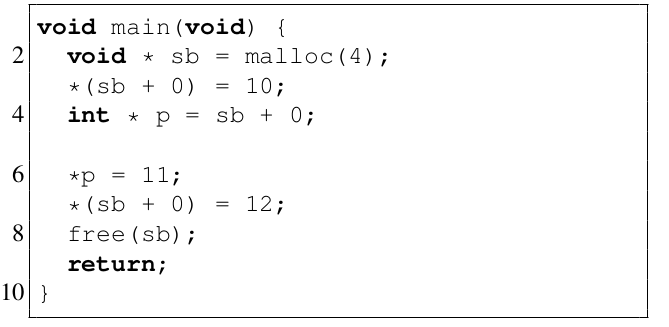
\includegraphics[scale=0.33]{images/after_shadow.png}
\caption{Malloc de la pile secondaire, le résultat est le code de droite (Joshua A. Kroll et al.)}
\label{shadow_stack}
\end{figure}


On voit ici que \texttt{i} aurait été placé sur la pile car il est adressé dans le code \texttt{\textbf{int}~*~p~=~\&i}. La transformation SFI fait en sorte qu'on alloue dynamiquement de la mémoire à \texttt{i} par un \texttt{malloc}, cette mémoire allouée est une trame de la pile secondaire. Il faut également que cette pile secondaire se situe dans la \textit{sandbox}. Pour cela on utilise en réalité un \texttt{malloc} qui a été réécrit dans le programme original pour utiliser une version SFI de \texttt{malloc}. Ainsi, les allocations mémoires dans le tas sont aussi redirigées vers la \textit{sandbox} par l'utilisation de ce \texttt{malloc}-SFI.

	\item \textit{Masquage des accès mémoires}, on masque toutes les opérations qui sont potentiellement illégales avec la fonction \textit{mask} présentée auparavant.
	
	\item \textit{Masquage des appels de fonctions}, des blocs mémoire sont spécialement réservés pour identifier les pointeurs de fonction. Chaque bloc identifie la signature d'une fonction et contient du code pour effectuer un appel vers la fonction concernée. De ce fait les pointeurs de fonction sont masqués et pointent vers ces blocs spéciaux. Ainsi, les interactions entre le module à risque et le programme sont contrôlées dans ces blocs.

	\item \textit{Production d'un code sémantiquement bien défini}, on veut que tous les programmes transformés aient une sémantique bien définie. Pour cela, on modifie le Cminor pour se protéger des opérations non définies sémantiquement. Par exemple, les variables locales qui apparaissent dans le module sont initialisées, on se protège des éventuelles divisions pas 0 par des vérifications à l'exécution, ou on vérifie que les appels de fonction correspondent bien à une signature existante. 
	
\end{itemize}

\subsubsection{\'Evaluation de l'approche}

Tout d'abord un point fort de cette approche est qu'elle possède une petite \textit{Trusted Computing Base}. En effet, pour que l'approche SFI-CompCert soit valide nous n'incluons dans la TCB que quelques éléments. Pour commencer, on suppose que les transformations SFI utilisées ne change pas le comportement du module à risque, ces transformations sont donc dans la TCB. Ensuite tout ce qui touche CompCert est également dans la TCB, en particulier les éléments non prouvés de CompCert tels que l'assistant à la preuve Coq ou l'assembleur utilisé pour obtenir un binaire du module à risque. En lien avec la TCB, nous avons aussi l'atout de pouvoir éviter l'implémentation d'un vérifieur pour chaque architecture ciblée.

Cette méthode de SFI a également d'autres avantages. Par exemple, les transformations sont portables sur toutes les architectures supportées par CompCert. De plus, les transformations se font sur le langage relativement haut niveau Cminor. De ce fait, les transformations introduites par SFI profitent des optimisations réalisées par CompCert ce qui améliorent les performances du module à risque.

Les performances obtenues par les expériences sont similaires à un compromis entre \texttt{gcc -O0} et \texttt{gcc -O1} pour les architectures ARM et x86. En comparant avec du code produit par CompCert sans modifications, on a une baisse de performance moyenne de 21,7\% sur x86 et 16,8\% sur ARM. 

Cependant l'approche SFI-CompCert a aussi des désavantages. Premièrement, les propriétés de correction de SFI ne s'appliquent pas pour des programmes concurrents. En effet, CompCert n'a pas de sémantique opérationnelle pour les programmes multi-tâches. Ensuite l'approche CompCert-SFI nous oblige à compiler les modules à risque pour avoir un exécutable \textit{sandboxé}. Dans l'approche classique le module à risque peut-être distribué sous forme de binaire, il suffit ensuite que le vérifieur le valide pour pouvoir l'exécuter sans danger.

\section{Objet du stage}

Dans la continuation de cette bibliographie je vais introduire la problématique sur laquelle je souhaiterais me pencher dans les mois à venir ainsi qu'une approche qui pourrait répondre à ces problèmes.

\subsection{Problématique}

On a vu que les techniques de SFI confinaient les sauts dans la mémoire de manière différente selon le mode d'adressage. Pour un adressage direct, le générateur de code réécrit directement les adresses de destination durant la compilation. Pour les adressages indirects on introduit des instructions de masquage pour que l'adresse stockée dans le registre durant l'exécution appartiennent à la \textit{sandbox}. Cependant, il existe une instruction de saut indirecte qui n'utilise pas les registres pour son adresse de destination, l'instruction de retour d'une fonction \texttt{ret}. 
Sachant que \texttt{ret} ne se sert pas des registres on ne peut pas masquer l'adresse de retour. On pourrait masquer la valeur stockée dans la pile, toutefois on serait toujours vulnérable à un problème de concurrence. En effet, on ne peut pas garantir que l'adresse de retour qu'on aura masquée ne sera pas réécrite pas un autre \textit{thread} avant d'appeler l'instruction \texttt{ret}. Le code est alors vulnérable aux attaques de type \textit{buffer overflow} qui écrasent les adresses de retour stockées dans la pile pour dévier le flot d'exécution du programme à leur avantage.
Dans les différents travaux présentés seuls Pittsfield~\cite{Mccamant_evaluatingsfi} et Native~Client~\cite{Yee:2010:NCS:1629175.1629203} s'intéressent à cette problématique. La solution proposée consiste à décomposer l'instruction \texttt{ret} par la combinaison d'un \texttt{pop}, pour dépiler une trame de la pile, et d'un \texttt{jmp} pour sauter au point de retour de la fonction. Cette solution est simple et fonctionne, il suffit de placer les opérations de \textit{sandboxing} avant le \textit{jmp} pour \textit{sandboxé} le module. Cependant les architectures modernes utilisent de nombreuses optimisations liées à l'instruction \texttt{ret} et la remplacer baisse les performances du module à risque.

%SFI utilise le \textit{sandboxing} pour réécrire les adresses de destination des instructions dangereuses. Ainsi, si une adresse pointe hors de la mémoire du module, ses bits de poids forts seront remplacés et désignera une adresse de la \textit{sandbox}. Cependant, nous n'avons aucune connaissance sur cette nouvelle adresse. En effet, celle-ci peut appartenir à une région de la mémoire non initialisée ou peut pointer sur des valeurs critiques du module. De ce fait, le flot de contrôle du module à risque est modifié et plus aucune garantie ne peut être faite sur son exécution.

\subsection{Approche proposée}

 L'idée principale est d'imposer à la pile des trames de taille constante. Ainsi les locations des adresses de retour dans la pile seront connues car elles seront séparées par des trames de taille constante. Le premier avantage sera qu'on pourra préserver l'intégrité de la pile. Supposons qu'une adresse de retour est situé à l'adresse $a$ et que les trames sont de taille $n$. Si on interdit toutes les écritures dans les adresses valant $a$ \% $n$ on protège alors toutes les adresses de retour de la pile. On peut de la même manière protéger toutes les zones d'une trame et notamment prévenir les \textit{buffer overflow}. De plus, les écritures dans la pile pourront être contrôlées par une interface faisant partie de notre TCB, ce qui nous donnera un contrôle plus fin sur les valeurs introduites dans la pile. Ce contrôle couplé à l'intégrité de la pile pourrait nous permettre d'optimiser les techniques de SFI. En effet, on pourrait au lieu de \textit{sandboxé} chaque accès aux valeurs de la pile, se contenter de \textit{sandboxé} ces valeurs au moment de leur écriture dans la pile, dans notre interface de confiance. L'intégrité de la pile étant préservée nous aurons alors la garantie que les adresses contenues dans la pile appartiennent bien à la \textit{sandbox}. On pourra alors éviter le \textit{sandboxing} lorsqu'on utilise des adresses sauvegardées dans la pile ce qui pourrait apporter un gain des performances.
 
	Pour réaliser cette approche nous faisons le choix d'utiliser CompCert. Ce choix pourrait à terme, nous permettre de prouver la légitimité des opérations que nous introduirons. Pour l'implémentation il faudra également choisir à quel niveau nous effectuerons les transformations. En faisant les transformations sur un langage de bas niveau comme l'assembleur la démarche est directe, cependant l'implémentation risque d'être délicate. En utilisant Cminor comme l'approche précédente, nous bénéficierons d'une vision plus simple de la problématique et l'analyse peu aussi être plus aisée. Toutefois il faudra s'assurer que les transformations soient sémantiquement bien définies dans le reste de la chaîne de la compilation. Ce choix nécessitera plus d'études sur le sujet et une meilleure compréhension des avantages et désavantages des deux propositions citées.

\section{Conclusion}

Nous avons présenté différentes implémentations de \textit{Software Fault Isolation} au cours de cette bibliographie. Toutes sont inspirées du travail fondateur de Wahbe et al.~\cite{Wahbe:1993:ESF:173668.168635} dans lequel les grands principes de la SFI sont établis. Les techniques de SFI ont pour but de confiner n'importe quel module à risque dans une \textit{sandbox} afin de prévenir les effets de bords éventuels sur le programme principal. Les techniques de SFI, lorsqu'elles sont appliquées sur un module respectant déjà ces principes, ne doivent pas changer le comportement de ce module.
Pour l'implémentation des techniques de SFI nous avons vu deux approches possibles. La première définie comme l'approche classique est composé d'un générateur de code et est suivi d'un vérifieur appartenant à la TCB. La deuxième méthode utilise un générateur de code couplé avec le compilateur certifié CompCert.

\textit{Software Fault Isolation} permet d'avoir des garanties de sécurité sur l'exécution d'un module à risque. En contrepartie les performances de ces modules sont plus basses que pour des modules intouchés. Pour limiter les ralentissements occasionnés, des optimisations peuvent être appliquées à l'aide d'analyses statiques~\cite{Abadi:2009:CIP:1609956.1609960}\cite{Zeng:2011:CCI:2046707.2046713}.
Par exemple, une instruction d'écriture dans une boucle exécutera le \textit{sandboxing} à chaque tour même si l'adresse de destination n'est pas modifiée. Une analyse statique peut détecter ce problème et proposerait de faire le \textit{sandboxing} avant la boucle évitant ainsi des opérations inutiles.

Durant notre stage de recherche nous voulons nous intéresser à une certaine problématique que présente SFI. En effet SFI ne spécifie pas de solutions concrètes pour la protection des adresses de retour stockées dans la pile. Pour répondre à ce problème nous proposons une approche basée sur des trames de pile de taille constante. Ainsi nous aurons un contrôle plus fin sur les valeurs stockées dans la pile et nous pourrons protéger les adresses de retour. Cette idée nous permettrait de nous protéger des attaques de type \textit{buffer overflow} qui dévient le flot de contrôle des programmes en modifiant les adresses de retour de la pile. Durant le stage nous essaierons de proposer une implémentation de cette approche.
  
%\nocite{Abadi:2009:CIP:1609956.1609960}
%\nocite{Ansel:2011:LSJ:1993316.1993540}
\bibliography{ref}
\bibliographystyle{plain}

\end{document}
%%% Local Variables:
%%% mode: latex
%%% TeX-master: t
%%% End:

